\subsection{Görbe közelítési módszerek: természetes spline, Bezier, Catmull-Rom görbék.}

Lényegük, hogy alakzatokat tudjunk leírni különböző módszerekkel

\textbf{3D görbék:}
\begin{itemize}
    \item függvényközelítés: $y = f(x)$, $z = g(x)$
    \item implicit görbemegadás: $f(x,y,z) = 0$
\end{itemize}

\textbf{Paraméteres görbemegadás:}
\begin{itemize}
    \item $x = x(t)$
    \item $y = y(t)$
    \item $z = z(t)$
    \item $t \in [t_0, t_1]$
\end{itemize}

\textbf{Geometriai folytonosság:}

$G^0 \implies x(t) \in C^0, y(t) \in C^0, z(t) \in C^0$

$G^1 \implies$ az érintők iránya folytonos $C^1 \neq G^1$

\begin{center}
    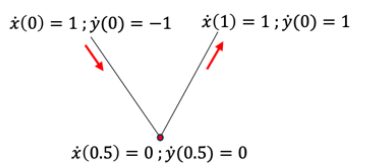
\includegraphics[width=0.4\textwidth]{res/imgs/info_22_geometric_continuity.png}
\end{center}

\textbf{Elsőfokú paraméteres görbeszakasz közelítés:}
\begin{minipage}{0.2\textwidth}
    \begin{center}
        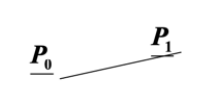
\includegraphics[width=\textwidth]{res/imgs/info_22_linear_curve.png}
    \end{center}
\end{minipage}
\begin{minipage}{0.4\textwidth}
    \begin{align*}
        \underline{Q}(t) &= \underline{P_0} + t \cdot (\underline{P_1} - \underline{P_0}) \\
        \underline{Q}(t) &= \underline{P_0} \cdot (1 - t) + \underline{P_1} \cdot t
    \end{align*}
\end{minipage}
\begin{minipage}{0.3\textwidth}
    \begin{center}
        $t \in [0, 1]$ \\
        $t \in [0, 1]$
    \end{center}
\end{minipage}

\begin{minipage}{0.3\textwidth}
    Súlyfüggvények:
    \begin{align*}
        S_0 &= -t + 1 \\
        S_1 &= t
    \end{align*}
\end{minipage}
\begin{minipage}{0.4\textwidth}
    \begin{center}
        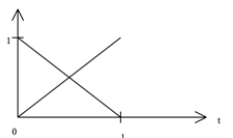
\includegraphics[width=\textwidth]{res/imgs/info_22_weights_linear.png}
    \end{center}
\end{minipage}

\begin{equation*}
    \underline{Q}(t) = \begin{bmatrix} Q_x(t) \\ Q_y(t) \\ Q_z(t) \end{bmatrix} = \begin{bmatrix} P_{0x} & P_{1x} \\ P_{0y} & P_{1y} \\ P_{0z} & P_{1z} \end{bmatrix} \begin{bmatrix} S_0 \\ S_1 \end{bmatrix} = \begin{bmatrix} P_{0x} & P_{1x} \\ P_{0y} & P_{1y} \\ P_{0z} & P_{1z} \end{bmatrix} \begin{bmatrix} -1 & 1 \\ 1 & 0 \end{bmatrix} \begin{bmatrix} t \\ 1 \end{bmatrix} \quad t \in [0,1]
\end{equation*}

\begin{equation*}
    \underline{Q}(t) = \underline{\underline{P}} * \underline{\underline{M}} * \underline{T}
\end{equation*}
Hol $\underline{\underline{P}}$ a Geometriát jellemző mátrix, $\underline{\underline{M}}$ a Bázismátrix, $\underline{T}$ a Paramétervektor.

\begin{itemize}
    \item egyenes egyenlete térben, $t$ a futó paraméter -- megszabja, mettől meddig menjen
\end{itemize}

\textbf{Harmadfokú paraméteres görbeszakasz közelítés -- Hermite-féle görbeszakasz:}
\begin{minipage}{0.7\textwidth}
    \begin{equation*}
        \underline{Q}(t) = \underline{P_1} * s_{P1}(t) + \underline{P_4} * s_{P4}(t) + \underline{R_1} * s_{R1}(t) + \underline{R_4} * s_{R4}(t) \quad t \in [0,1]
    \end{equation*}
    \begin{itemize}
        \item egy függvényhez -- görbéhez 4 adat kell
        \item a kezdő- és végpont koordinátái
        \item valamint a kezdő- és végpontokba húzott érintő egyenes egyenletei (vektorosan)
    \end{itemize}
\end{minipage}
\begin{minipage}{0.2\textwidth}
    \begin{center}
        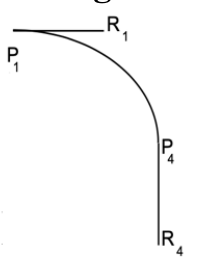
\includegraphics[width=\textwidth]{res/imgs/info_22_hermite.png}
    \end{center}
\end{minipage}

\textbf{Bezier-féle görbeszakasz:}
\begin{minipage}{0.6\textwidth}
    \begin{itemize}
        \item Hermite módszeréhez hasonló, viszont nem az érintő vektorát adjuk meg, hanem még 1-1 pontot, melyeket a kezdő- és végpontokkal összekötve megkapjuk az azokba húzott érintő egyenest.
    \end{itemize}
\end{minipage}
\begin{minipage}{0.3\textwidth}
    \begin{center}
        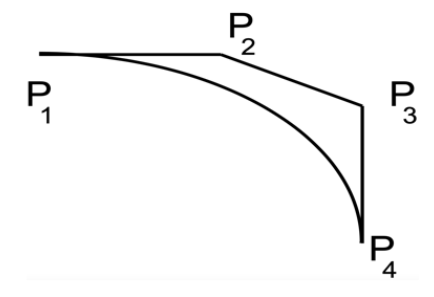
\includegraphics[width=\textwidth]{res/imgs/info_22_bezier.png}
    \end{center}
\end{minipage}

\textbf{Kardinális spline -- Catmull-Rom görbék:}
\begin{center}
    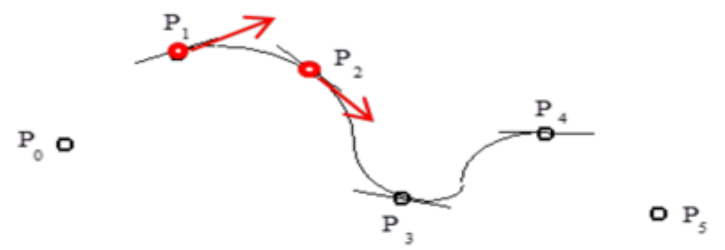
\includegraphics[width=0.6\textwidth]{res/imgs/info_22_catmull_rom.png}
\end{center}
\begin{equation*}
    \underline{V_k} = \tau \cdot (\underline{P_{k+1}} - \underline{P_{k-1}})
\end{equation*}
A $\tau = (1 - f)$, ahol $f \le 1$ a görbe feszítése. Ha $f = 0$, akkor $\tau = 1$, az éppen a Catmull-Rom spline.
\begin{itemize}
    \item interpoláló görbe
    \item Hermite-féle görbeszakaszból származtatott
    \item a pontokhoz tartozó érintővektorokat a szomszédos pontokból számolja
    \item f: kardinális paraméter -- mennyire sima/szögletes a görbe
\end{itemize}

\textbf{Természetes spline:}
\begin{center}
    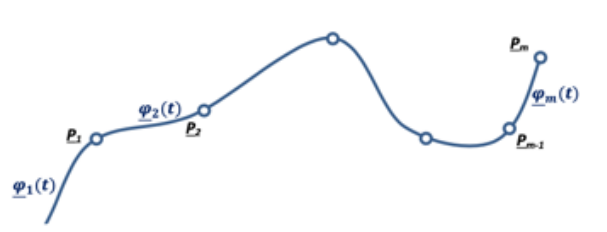
\includegraphics[width=0.8\textwidth]{res/imgs/info_22_natural_spline.png}
\end{center}
\begin{center}
    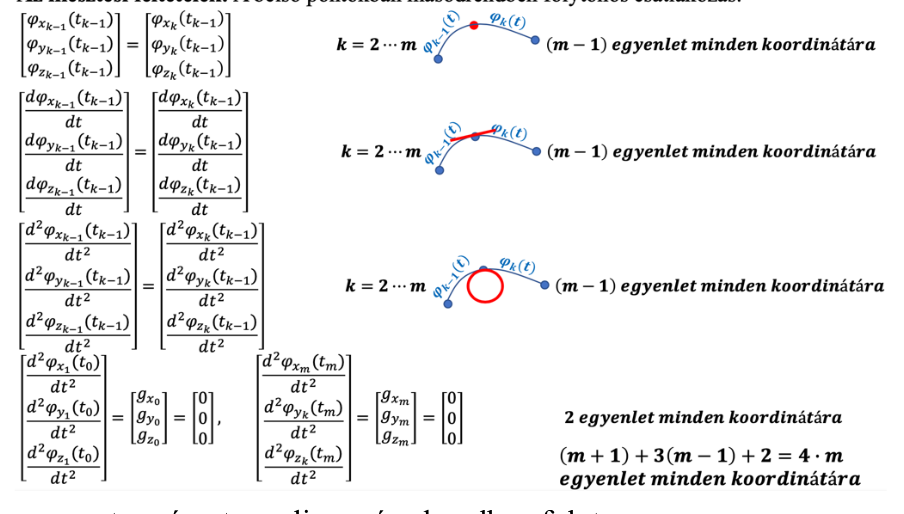
\includegraphics[width=0.95\textwidth]{res/imgs/info_22_natural_spline_eq.png}
\end{center}

\begin{itemize}
    \item természetes spline másodrendben folytonos
    \item végei kiegyenesednek
\end{itemize}